\documentclass{article}
\usepackage[utf8]{inputenc}
\usepackage{fullpage,amsmath,hyperref,indentfirst,graphicx,wrapfig,caption,subcaption}
\graphicspath{{~/Desktop/JUPYTER-LAB}}
\date{}
\begin{document}
{\LARGE{\hskip 2.2 in CS170 Project 1}}
\vskip 0.5in
{\flushleft{Brandon Paulsen}}
{\flushleft{October 31$^\text{st}$, 2022}}
{\flushleft{UCR CS170 Fall 2022}}
{\flushleft{Professor Eamonn Keough}}
\vskip 0.5in
\tableofcontents
\listoffigures
\pagebreak
\section{Introduction}
In this project, we are asked to write a program that uses a general search algorithm (A*) to solve 8 puzzles. An 8 puzzle is a puzzle that has 8 tiles arranged in a 3x3 grid, with one space. The goal of the puzzle is to arrange the tiles such that the first row is [1,2,3], the second row is [4,5,6], and the last row is [7,8,empty] by moving tiles around. Tiles next to the empty tile can swap places with the empty tile, or we can understand this as the empty tile swapping with tiles next to it.
\par A* is a search agorithm that uses both the depth of a state and a heuristic function to gague which unexplored states in the frontier should be explored first. It does this by assigning each state in the frontier a priority that is equal to the sum of the depth and heuristic, and as long as the heuristic is admissible (that is, it never overestimates the number of moves from the state to the goal state), A* will be optimal. In this project, we are tasked with implementing 3 heuristic functions: Uniform Cost, Misplaced Tiles, and Manhattan Distance.
\par As has been discussed in class multiple times, the branching factor and diameter of a search problem are very important. In fact, the branching factor and the problem diameter of a search problem define the magnitude of the search space, so it might be good to investigate them a little bit. Based on the loose idea that the branching factor is the average of the number of valid moves of a state, we can approximate the branching factor as $4\cdot\frac{1}{9}+3\cdot\frac{4}{9}+2\cdot\frac{4}{9} = \frac{24}{9} \approx 2.6$, because there are 4 corner spaces with 2 moves, 4 edge spaces with 3 moves, and 1 center space with 4 moves. This seems reasonable, but if we further consider that we cannot go back to any states previously visited, and at least one move for each state goes back to a previous state, we can reduce the approximate branching factor to $3\cdot\frac{1}{9}+2\cdot\frac{4}{9}+1\cdot\frac{4}{9} = \frac{15}{9} \approx 1.7$. This is a very small branching factor, which is great news for us. We can further extend this approximation of the branching factor to any n puzzle as $\frac{4}{n^2}+\frac{8\cdot(n-2)}{n^2}+\frac{3\cdot(n^2-4\cdot(n-2)-4)}{n^2} = 3-\frac{4}{n}$.
\section{Heuristics}
Heuristics are a the heart of the A* algorithm, without them, A* would be no better than breadth first search. As such, it is important to discuss the heuristics used in this project both in terms of their implementation and their impact on space and time complexity.
\subsection{Uniform Cost}
Uniform Cost Heuristic is the simplest of the 3 heuristics. It simply evaluates to 0 for all states. This means that in effect, A* with Uniform Cost Heuristic devolves to breadth first search and searches level-by-level. This clearly implies that the algorithm will be complete and optimal, though it will be very slow and memory inefficient as well.
\subsection{Misplaced Tile}
Misplaced Tile Heuristic, though slightly more complex than Uniform Cost Heuristic (which is trivial), is not overly complex. Evaluating the Misplaced Tile Heuristic of a state amounts to counting up the number of tiles in a given state that are not in the same position as they are in the goal state. Though it is much better than Uniform Cost Heuristic, it is clearly not the best heuristic (either in terms of time or memory), as children of a state (those states that are reachable from that state in a move) often are assigned the same priority, and therefore the search algorithm has a hard time distinguishing which is better and should be explored first.
\pagebreak
\subsection{Manhattan Distance}
Though Manhattan Distance Heuristic is the most complex of the 3, it offers some potential benefits that warrant its use. In all cases, Manhattan Distance Heuristic dominates Misplaced Tile Heuristic - that is to say, its value is greater than Misplaced Tile Hueristic without overestimating the number of moves left and therefore destroying the optimality of the A* algorithm. The Manhattan Distance Heuristic is calculated by totaling the differences in x and y positions of tiles between a given state and the goal state, or in math terms, $\sum_{\text{tiles}\neq\text{empty}}\Delta x + \Delta y$. Though Manhattan Distance Heuristic is admissible, it is clearly not perfect, and there is still room for improvement.
\section{Test Cases}
Several cases were given in the project assignment. They range from trivial (depth 0) to very complex (depth 24) and make for good tests of algorithms. For a significant portion of time, my implementation of the general search algorithm when used with Manhattan Distance Heuristic failed to find the most optimal path (the path it found was at depth 26). This was very helpful to me in that it indicated an error in my code. The number of vistied nodes, frontier nodes, and searh time trends are plotted below for each heuristic:
\begin{figure}[ht]
	\centering
	\begin{subfigure}[b]{0.32\textwidth}
		\centering
		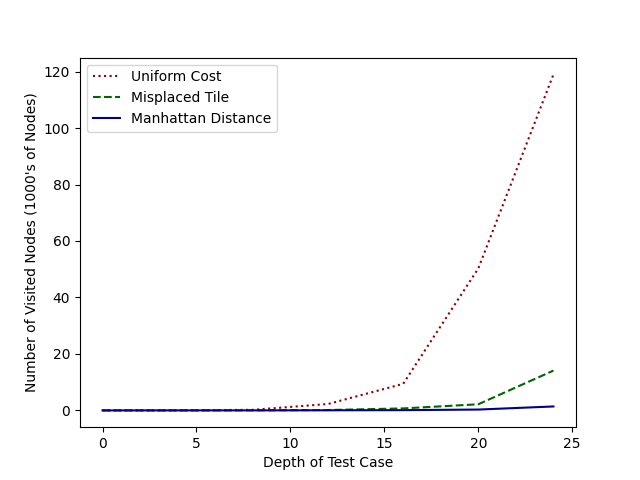
\includegraphics[width = \textwidth]{testVisitedComparison.png}
		\caption{Visited Nodes vs Depth}
		\label{fig:Visited Nodes Comparison}
	\end{subfigure}
	\hfill
	\begin{subfigure}[b]{0.32\textwidth}
		\centering
		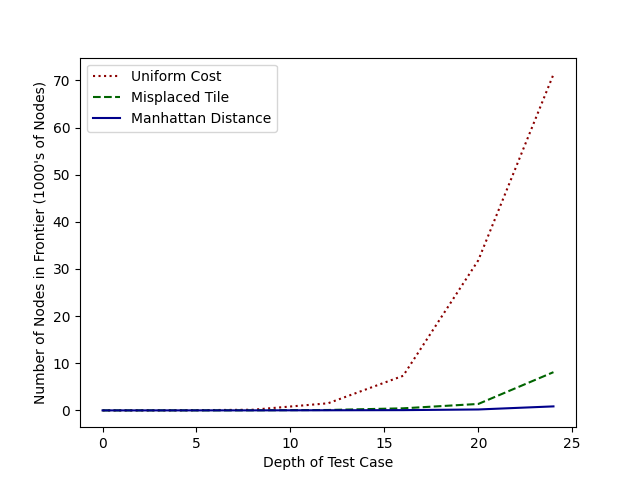
\includegraphics[width = \textwidth]{testFrontierComparison.png}
		\caption{Frontier Nodes vs Depth}
		\label{fig:Frontier Nodes Comparison}
	\end{subfigure}
	\hfill
	\begin{subfigure}[b]{0.32\textwidth}
		\centering
		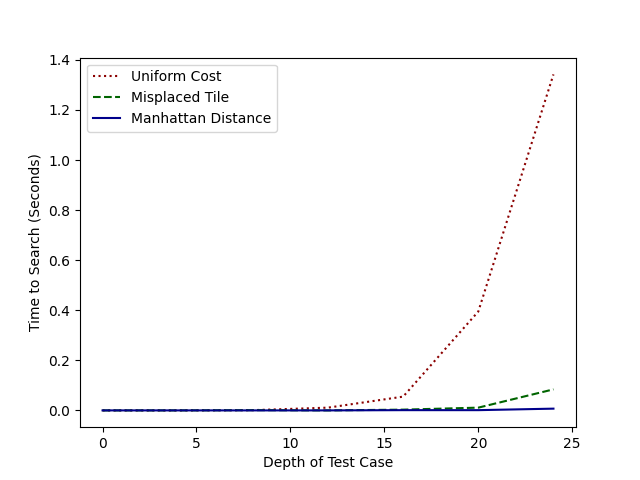
\includegraphics[width = \textwidth]{testTimeComparison.png}
		\caption{Search Time vs Depth}
		\label{fig:Search Time Comparison}
	\end{subfigure}
	\caption{Test Cases Trend Comparisons}
	\label{fig:Test Cases Trend Comparisons}
\end{figure}
\par It is important to note that even though the Manhattan Distance trends seem linear, they are very much not (as can be seen in Figure \ref{fig:Manhattan Distance Monte Carlo Simulation}). 
\section{Monte Carlo Simulation}
I ran a monte carlo simulation with 100,000 trials to get some idea of how the number of visited nodes, frontier nodes, and search time changed with depth for each heuristic. Running 100,000 trials of Manhattan Distance search is unfeasible in python, let alone uniform cost, so I wrote the monte carlo simulation in my C++ implementation. Overall, the trials took something like a few hours to run the simulation, most of which was due to the uniform cost search, but it was well worth it to satisfy my curiousity.  For each heuristic, I recorded the number of visited states, number of frontier states at the time of finding the goal state (though there may have been more goal states previously), and the amount of time that the search took, all as an average per depth.
\pagebreak
\subsection{Uniform Cost}
Below are the plotted results of my monte carlo sumulation of the Uniform Cost Heuristic:
\begin{figure}[ht]
	\centering
	\begin{subfigure}[b]{0.32\textwidth}
		\centering
		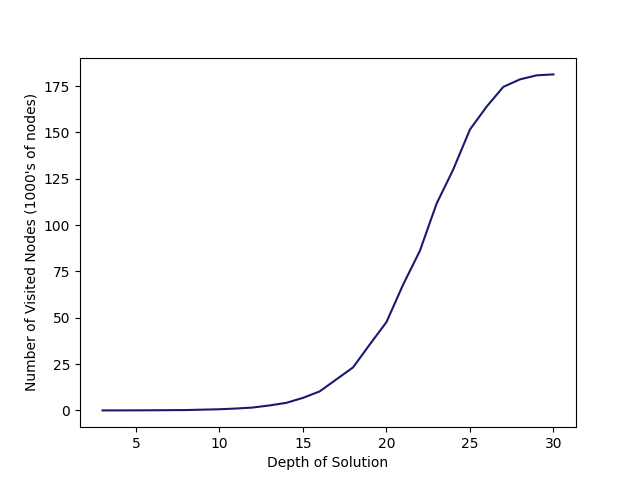
\includegraphics[width = \textwidth]{uniformCostVisited.png}
		\caption{Visited Nodes vs Depth}
		\label{fig:Uniform Cost Visited Nodes}
	\end{subfigure}
	\hfill
	\begin{subfigure}[b]{0.32\textwidth}
		\centering
		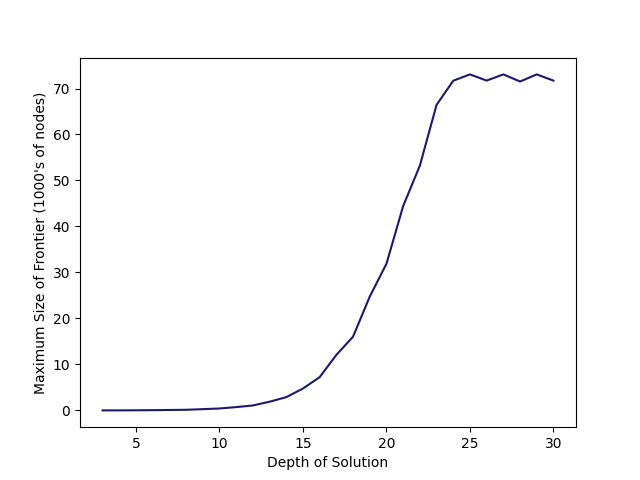
\includegraphics[width = \textwidth]{uniformCostFrontier.png}
		\caption{Frontier Nodes vs Depth}
		\label{fig:Uniform Cost Frontier Nodes}
	\end{subfigure}
	\hfill
	\begin{subfigure}[b]{0.32\textwidth}
		\centering
		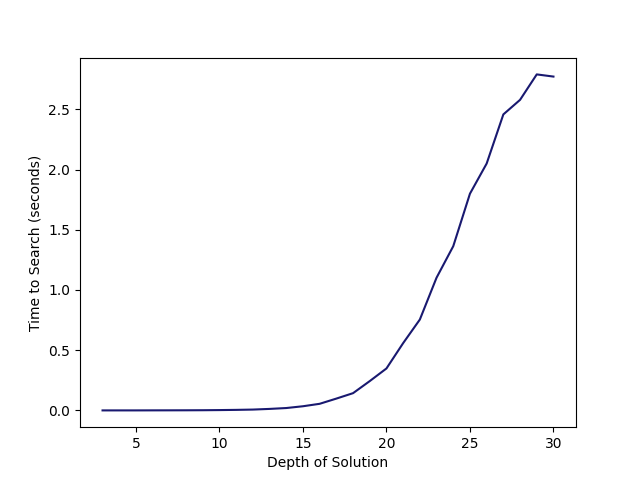
\includegraphics[width = \textwidth]{uniformCostTime.png}
		\caption{Search Time vs Depth}
		\label{fig:Uniform Cost Search Time}
	\end{subfigure}
	\caption{Uniform Cost Monte Carlo Simulation Results}
	\label{fig:Uniform Cost Monte Carlo Simulation}
\end{figure}
\par In these graphs, it can be seen that the number of visited nodes, the number of frontier nodes, and the search trime grow approximately exponentially (as should be expected), but taper off significantly as the depth nears the diameter of the problem. This is because, as we get closer and closer to the maximum possible depth, we have already explored most of the possible states of the puzle and there are less to explore, decreasing the branching factor quite significantly. If this were not the case, we would expect to see the Uniform Cost Visited Nodes exponential trend continue indefinitely.
\subsection{Misplaced Tile}
Below are plotted the results of my monte carlo simulation of the Misplaced Tile Heuristic:
\begin{figure}[h]
	\centering
	\begin{subfigure}[b]{0.32\textwidth}
		\centering
		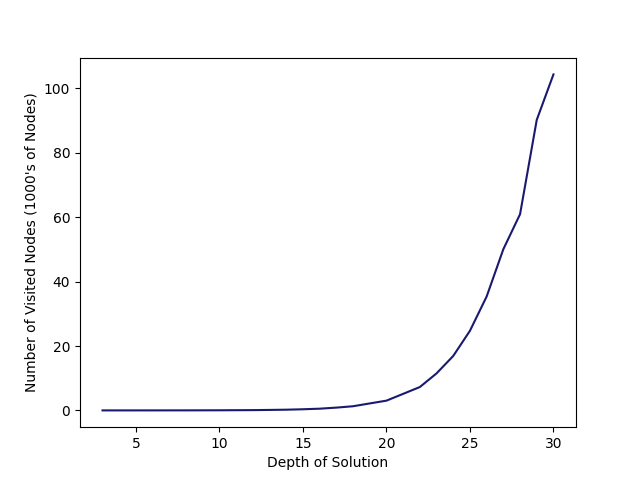
\includegraphics[width = \textwidth]{misplacedTileVisited.png}
		\caption{Visited Nodes vs Depth}
		\label{fig:Misplaced Tile Visited Nodes}
	\end{subfigure}
	\hfill
	\begin{subfigure}[b]{0.32\textwidth}
		\centering
		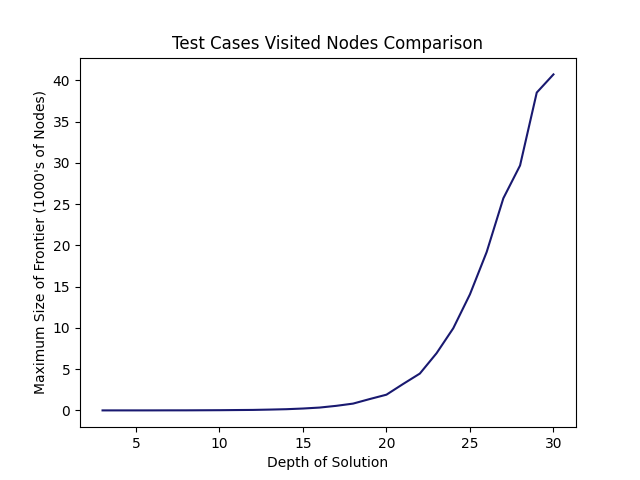
\includegraphics[width = \textwidth]{misplacedTileFrontier.png}
		\caption{Frontier Nodes vs Depth}
		\label{fig:Misplaced Tile Frontier Nodes}
	\end{subfigure}
	\hfill
	\begin{subfigure}[b]{0.32\textwidth}
		\centering
		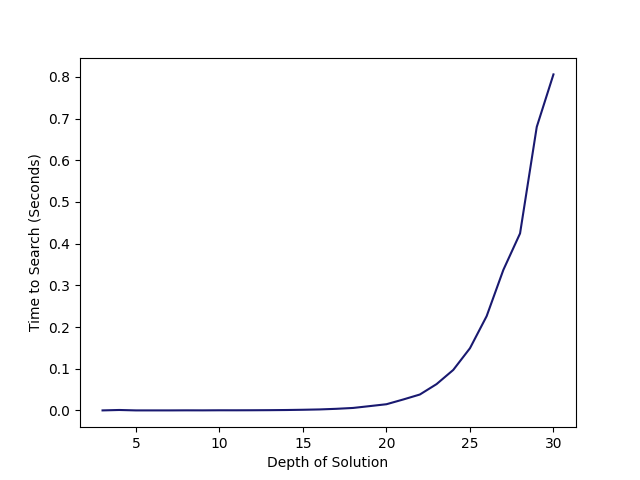
\includegraphics[width = \textwidth]{misplacedTileTime.png}
		\caption{Search Time vs Depth}
		\label{fig:Misplaced Tile Search Time}
	\end{subfigure}
	\caption{Misplaced Tile Monte Carlo Simulation Results}
	\label{fig:Misplaced Tile Monte Carlo Simulation}
\end{figure}
\par Each of these graphs grows exponentially initially, but tapers off only slightly as the solution depth reaches the diameter of the solution (31). This is noteworthy, because as can be seen by comparing Figure \ref{fig:Misplaced Tile Frontier Nodes} and Figure \ref{fig:Uniform Cost Frontier Nodes}, the taper is much less, indicating that the Misplaced Tile Heurisic avoids exhaustively searching layer-by-layer.
\pagebreak
\subsection{Manhattan Distance}
Below are plotted the results of my monte carlo simulation of the Manhattan Distance Heuristic:
\begin{figure}[h]
	\centering
	\begin{subfigure}[b]{0.32\textwidth}
		\centering
		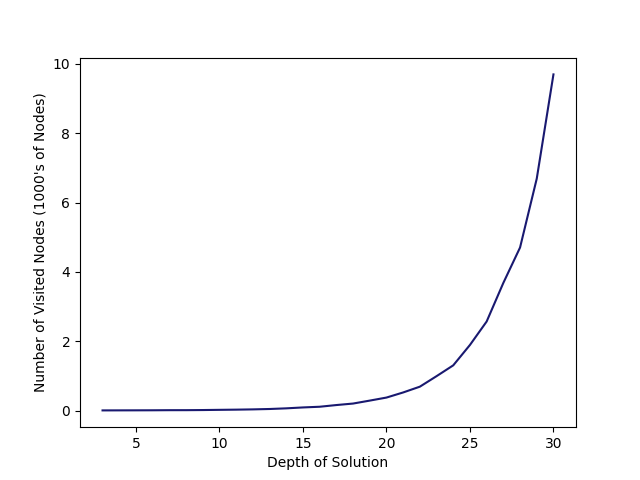
\includegraphics[width = \textwidth]{manhattanDistanceVisited.png}
		\caption{Visited Nodes vs Depth}
		\label{fig:Manhattan Distance Visited Nodes}
	\end{subfigure}
	\hfill
	\begin{subfigure}[b]{0.32\textwidth}
		\centering
		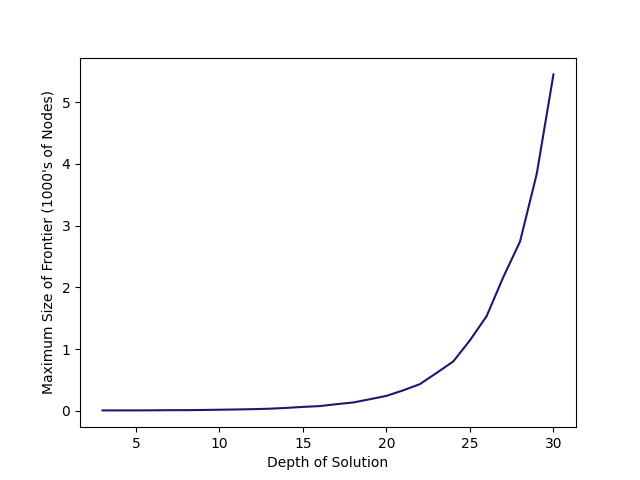
\includegraphics[width = \textwidth]{manhattanDistanceFrontier.png}
		\caption{Frontier Nodes vs Depth}
		\label{fig:Manhattan Distance Frontier Nodes}
	\end{subfigure}
	\hfill
	\begin{subfigure}[b]{0.32\textwidth}
		\centering
		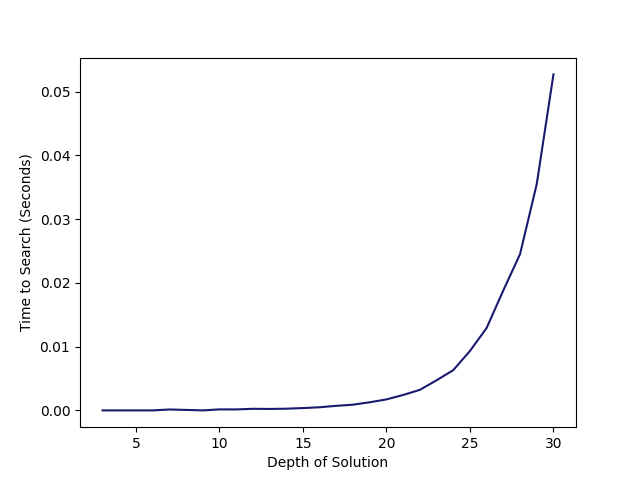
\includegraphics[width = \textwidth]{manhattanDistanceTime.png}
		\caption{Search Time vs Depth}
		\label{fig:Manhattan Distance Search Time}
	\end{subfigure}
	\caption{Manhattan Distance Monte Carlo Simulation Results}
	\label{fig:Manhattan Distance Monte Carlo Simulation}
\end{figure}
\par In comparing Figure \ref{fig:Manhattan Distance Search Time} and Figure \ref{fig:Uniform Cost Search Time}, both heuristics start off with similar search times for puzzle states close to the goal state, but quickly diverge in the search time. Overall, for very deep nodes (~30 deep), the Manhattan Distance search time becomes someting like 150 times faster on average. In addition, for deep nodes, Manhattan Distance Heuristic visits about 50 times fewer nodes as does the Uniform Cost Heuristic (Figure \ref{fig:Manhattan Distance Visited Nodes} vs Figure \ref{fig:Uniform Cost Visited Nodes}).
\subsection{Trend Comparison}
Below are plotted trend comparisons for the number of visited ndoes, the number of nodes in the frontier, and the search time vs depth for each heuristic:
\begin{figure}[ht]
	\centering
	\begin{subfigure}[b]{0.32\textwidth}
		\centering
		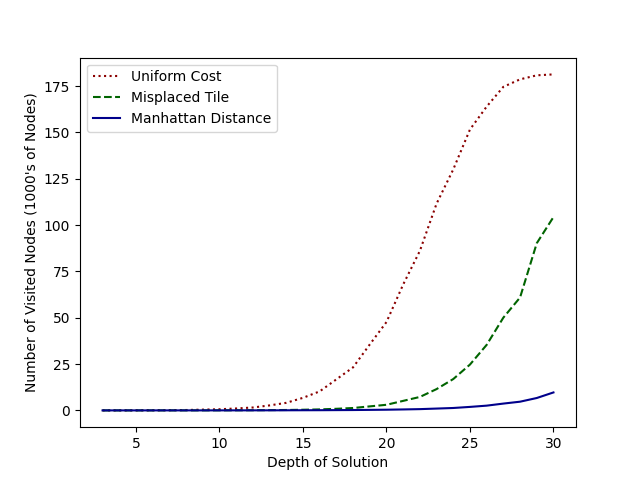
\includegraphics[width = \textwidth]{visitedComparison.png}
		\caption{Visited Nodes vs Depth}
		\label{fig:Visited Nodes Comparison}
	\end{subfigure}
	\hfill
	\begin{subfigure}[b]{0.32\textwidth}
		\centering
		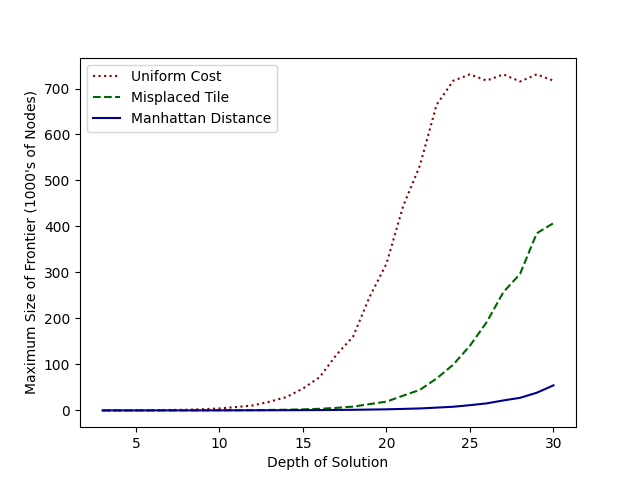
\includegraphics[width = \textwidth]{frontierComparison.png}
		\caption{Frontier Nodes vs Depth}
		\label{fig:Frontier Comparison}
	\end{subfigure}
	\hfill
	\begin{subfigure}[b]{0.32\textwidth}
		\centering
		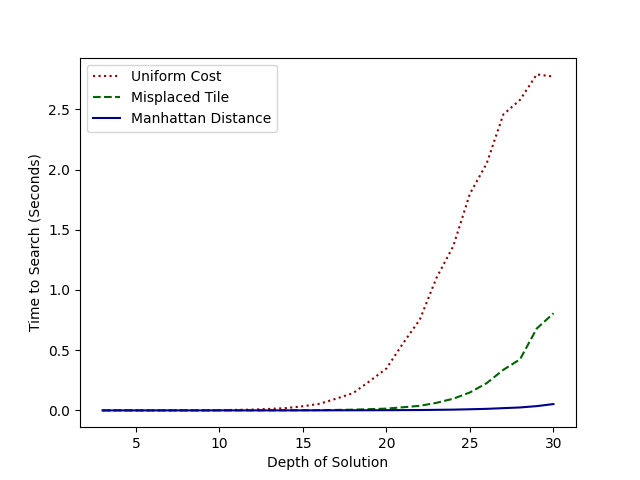
\includegraphics[width = \textwidth]{timeComparison.png}
		\caption{Search Time vs Depth}
		\label{fig:Search Time Comparison}
	\end{subfigure}
	\caption{Monte Carlo Simulation Trend Comparisons}
	\label{fig:Monte Carlo Trend Comparisons}
\end{figure}
\par We can clearly see that \emph{on average}, the Manhattan Distance Heuristic is much better in terms of runtime and memory complexity, especially as we solve deeper puzzles.
\pagebreak
\section{Conclusion}
In conclusion, through this project, we have seen that each heuristic is optimal and complete, though they vary in their runtimes and memory complexity. Each heuristic is exponential with respect to its time and space complexity, though the Manhattan Distance is clearly much faster and uses much less memory on average than the other two (as can be seen in Figure \ref{fig:Search Time Comparison} and Figure \ref{fig:Frontier Comparison}, respectively).
\par Though the code is capable of solving 15 puzzles currently (the object based C++ version), it takes somewhere on the order of 5-10 minutes, so I would want to modify it to implement island based search.  I would expect this to significantly speed up the search (though it would no longer be optimal), possibly to something on the order of 30-50 seconds.
\section{Code}
\subsection{C++}
My pointer based C++ code can be found at \url{https://github.com/Poly1581/SlidingPuzzles}
\par My object based C++ code can be found at \url{https://github.com/Poly1581/SlidingPuzzlesV2}
\subsection{Python}
My python code can be found at \url{https://github.com/Poly1581/PYSlidingPuzzles}


\end{document}
